\documentclass[12pt, a4paper]{article}
\usepackage[utf8]{inputenc}
\usepackage[english]{babel}
\usepackage{amsmath}
\usepackage{amsfonts}
\usepackage{amssymb}
\usepackage{siunitx}
\usepackage{longtable}
\usepackage[margin=1in]{geometry}
\usepackage{graphicx}
\usepackage{float}

\begin{document}

\begin{center}
	\Large \textbf{Experiment 1: Viscosity Coefficient of Glycerin}
	\vspace{0.5cm}
	    
	\normalsize Marmara University - Department of Physics \\
	Physics 3 Laboratory \\
	Experiment Report
	\vspace{0.5cm}
\end{center}

\section{Objective}
The purpose of this experiment is to measure the viscosity coefficient ($\eta$) of glycerin, a viscous liquid, by applying Stokes' Law. This involves observing the motion of steel balls falling through the liquid and calculating the viscosity based on their terminal velocities.

\section{Theoretical Background}
Imagine you have a small sphere, like a tiny steel ball, dropping slowly through a thick, syrupy liquid such as glycerin. Unlike dropping it in air, where it falls quickly, in glycerin, it moves very slowly due to the liquid's resistance. This resistance is called viscosity, which is a measure of how "sticky" or resistant the fluid is to flow.

Stokes' Law describes this phenomenon. It states that when a sphere moves through a viscous fluid at a constant speed (called the terminal velocity), the frictional force opposing the motion is given by:
\[ F_v = 6\pi \eta v r \]
where:
- $\eta$ is the viscosity coefficient of the fluid (what we're trying to measure),
- $v$ is the terminal velocity of the sphere,
- $r$ is the radius of the sphere.

To understand how we get to this, let's start from the beginning, as if explaining to someone new to physics.

When the sphere is first dropped, its initial speed is zero. At that moment, two main forces act on it: gravity pulling it down and buoyancy (the ascending force) pushing it up, due to the fluid it displaces.

The gravitational force is:
\[ F_g = m g = \frac{4}{3} \pi r^3 \rho_2 g \]
where $m$ is the mass of the sphere, $g$ is gravitational acceleration, $\rho_2$ is the density of the sphere (steel in this case), and $\frac{4}{3} \pi r^3$ is the volume.

The buoyant force, according to Archimedes' principle, is:
\[ F_a = \rho_1 V g = \frac{4}{3} \pi r^3 \rho_1 g \]
where $\rho_1$ is the density of the fluid (glycerin), and $V$ is the volume of the sphere (since it's fully submerged).

The net force downward initially is:
\[ F_{\text{net}} = F_g - F_a = \frac{4}{3} \pi r^3 (\rho_2 - \rho_1) g \]
This causes the sphere to accelerate downward with initial acceleration:
\[ a = \frac{F_{\text{net}}}{m} = \frac{\rho_2 - \rho_1}{\rho_2} g \]

As the sphere gains speed, the viscous drag force (Stokes' frictional force) starts to act upward, opposing the motion. This drag force increases with speed. Eventually, the drag force equals the net downward force, the acceleration becomes zero, and the sphere reaches a constant terminal velocity $v$.

At terminal velocity:
\[ F_v = F_g - F_a \]
\[ 6\pi \eta v r = \frac{4}{3} \pi r^3 (\rho_2 - \rho_1) g \]
Solving for $\eta$:
\[ \eta = \frac{2}{9} \frac{(\rho_2 - \rho_1) g r^2}{v} \]
This is the key formula we use. Note that $\rho_1$ is the mass density of the glycerin, and $\rho_2$ is the mass density of the steel balls.

\section{Apparatus and Method}
The materials used include:
- Glycerin as the viscous fluid,
- A 100 ml graduated cylinder to contain the glycerin,
- A thermometer to measure the temperature of the glycerin,
- Two steel balls with different diameters (0.47 cm and 0.30 cm),
- A stopwatch for timing the fall,
- A caliper to measure the diameters of the balls,
- A ruler to measure the distance between marks A and B,
- A magnet to release and retrieve the balls without disturbing the fluid.

The procedure was as follows:
1. The graduated cylinder was filled with glycerin, and we waited for any bubbles to dissipate.
2. The steel balls were cleaned by soaking in sodium hydroxide to remove grease and oil, then handled with tweezers.
3. The diameters of the balls were measured using the caliper, and radii were calculated.
4. Marks A and B were set at the 200 ml and 100 ml levels on the cylinder, corresponding to a distance $L = 7.4$ cm, measured with the ruler.
5. Using the magnet, each ball was released from the surface of the glycerin. The time taken to fall from A to B was recorded three times per ball using the stopwatch.
6. The temperature of the glycerin was measured with the thermometer and found to be 20°C.

This setup ensures the balls reach terminal velocity in the measured section, as the initial acceleration phase occurs earlier.

\section{Measurements and Data}
Constants used:
\begin{itemize}
	\item Density of steel balls ($\rho_2$): \SI{7870}{\kilo\gram\per\metre\cubed}
	\item Density of glycerin ($\rho_1$): \SI{900}{\kilo\gram\per\metre\cubed} (noted to be lower than typical pure glycerin density of about 1260 kg/m³, likely due to impurity)
	\item Gravitational acceleration ($g$): \SI{9.80}{\metre\per\second\squared}
	\item Distance between A and B ($L$): \SI{7.4}{\centi\metre} = \SI{0.074}{\metre}
	\item Temperature of glycerin ($T$): \SI{20}{\celsius}
\end{itemize}

The measurements are presented in the table below. Note that diameters and radii are initially in cm but converted to meters for SI unit consistency in calculations (e.g., $r$ in m for $r^2$ in m²).

\begin{small}
	\begin{longtable}{|c|c|c|c|c|c|c|c|c|c|}
		\caption{Glycerin Viscosity Measurement and Calculation} \label{tab:olcum} \\
		\hline
		\textbf{Ball} & \textbf{d} (\si{cm}) & \textbf{r} (\si{cm}) & \textbf{$r^2$} (\si{m^2}) & \multicolumn{3}{c|}{\textbf{Time, $t$} (\si{s})} & \textbf{$t_{avg}$} (\si{s}) & \textbf{$v$} (\si{m/s}) & \textbf{$\eta$} (\si{Pa.s}) \\
		\cline{5-7}
		  &        &         &                       & \textbf{$t_1$} & \textbf{$t_2$} & \textbf{$t_3$} &       &        &        \\
		\hline
		1 & 0.47 & 0.235 & $5.5225 \times 10^{-6}$ & 0.61           & 0.68           & 0.49           & 0.593 & 0.1248 & 0.6717 \\
		2 & 0.30 & 0.150 & $2.25 \times 10^{-6}$ & 1.73           & 1.72           & 1.64           & 1.70  & 0.0435 & 0.7851 \\
		\hline
		\multicolumn{9}{|r|}{\textbf{Mean $\eta_{avg}$}} & 0.7284 \\
		\hline
	\end{longtable}
\end{small}

\section{Calculations and Graphs}
The terminal velocity for each ball is calculated as $v = L / t_{\text{avg}}$, where $L = 0.074$ m.

For ball 1: $t_{\text{avg}} = (0.61 + 0.68 + 0.49)/3 = 0.593$ s, $v = 0.074 / 0.593 \approx 0.1248$ m/s

For ball 2: $t_{\text{avg}} = (1.73 + 1.72 + 1.64)/3 = 1.70$ s, $v = 0.074 / 1.70 \approx 0.0435$ m/s

The viscosity for each ball is then:
\[ \eta = \frac{2}{9} \frac{(\rho_2 - \rho_1) g r^2}{v} \]

For ball 1:
\[ \eta_1 = \frac{2}{9} \frac{(7870 - 900) \times 9.80 \times 5.5225 \times 10^{-6}}{0.1248} \approx 0.6717 \, \text{Pa·s} \]

For ball 2:
\[ \eta_2 = \frac{2}{9} \frac{(7870 - 900) \times 9.80 \times 2.25 \times 10^{-6}}{0.0435} \approx 0.7851 \, \text{Pa·s} \]

Average viscosity:
\[ \eta_{\text{avg}} = \frac{0.6717 + 0.7851}{2} = 0.7284 \, \text{Pa·s} \]

For the graphical method, we plot $v$ vs. $r^2$. From Stokes' Law, $v = \frac{2}{9} \frac{(\rho_2 - \rho_1) g}{\eta} r^2$, so the slope $m = \frac{2}{9} \frac{(\rho_2 - \rho_1) g}{\eta}$, and thus $\eta = \frac{2 (\rho_2 - \rho_1) g}{9 m}$.

The slope $m$ using the two points:
\[ m = \frac{0.1248 - 0.0435}{5.5225 \times 10^{-6} - 2.25 \times 10^{-6}} = \frac{0.0813}{3.2725 \times 10^{-6}} \approx 24844 \, \text{m}^{-1} \text{s}^{-1} \]

Then:
\[ \eta_{\text{graph}} = \frac{2 \times (7870 - 900) \times 9.80}{9 \times 24844} \approx 0.611 \, \text{Pa·s} \]

The viscosity at 18°C is corrected using the formula:
\[ \eta(18^\circ \text{C}) = \eta(T^\circ \text{C}) \left[1 + 0.026 (T - 18)\right] \]
For $T = 20^\circ$C, $\eta(20^\circ \text{C}) = 0.7284$ Pa·s:
\[ \eta(18^\circ \text{C}) = 0.7284 \times [1 + 0.026 \times (20 - 18)] = 0.7284 \times 1.052 \approx 0.766 \, \text{Pa·s} \]

\subsection{Graph}
\begin{figure}[H]
	\centering
	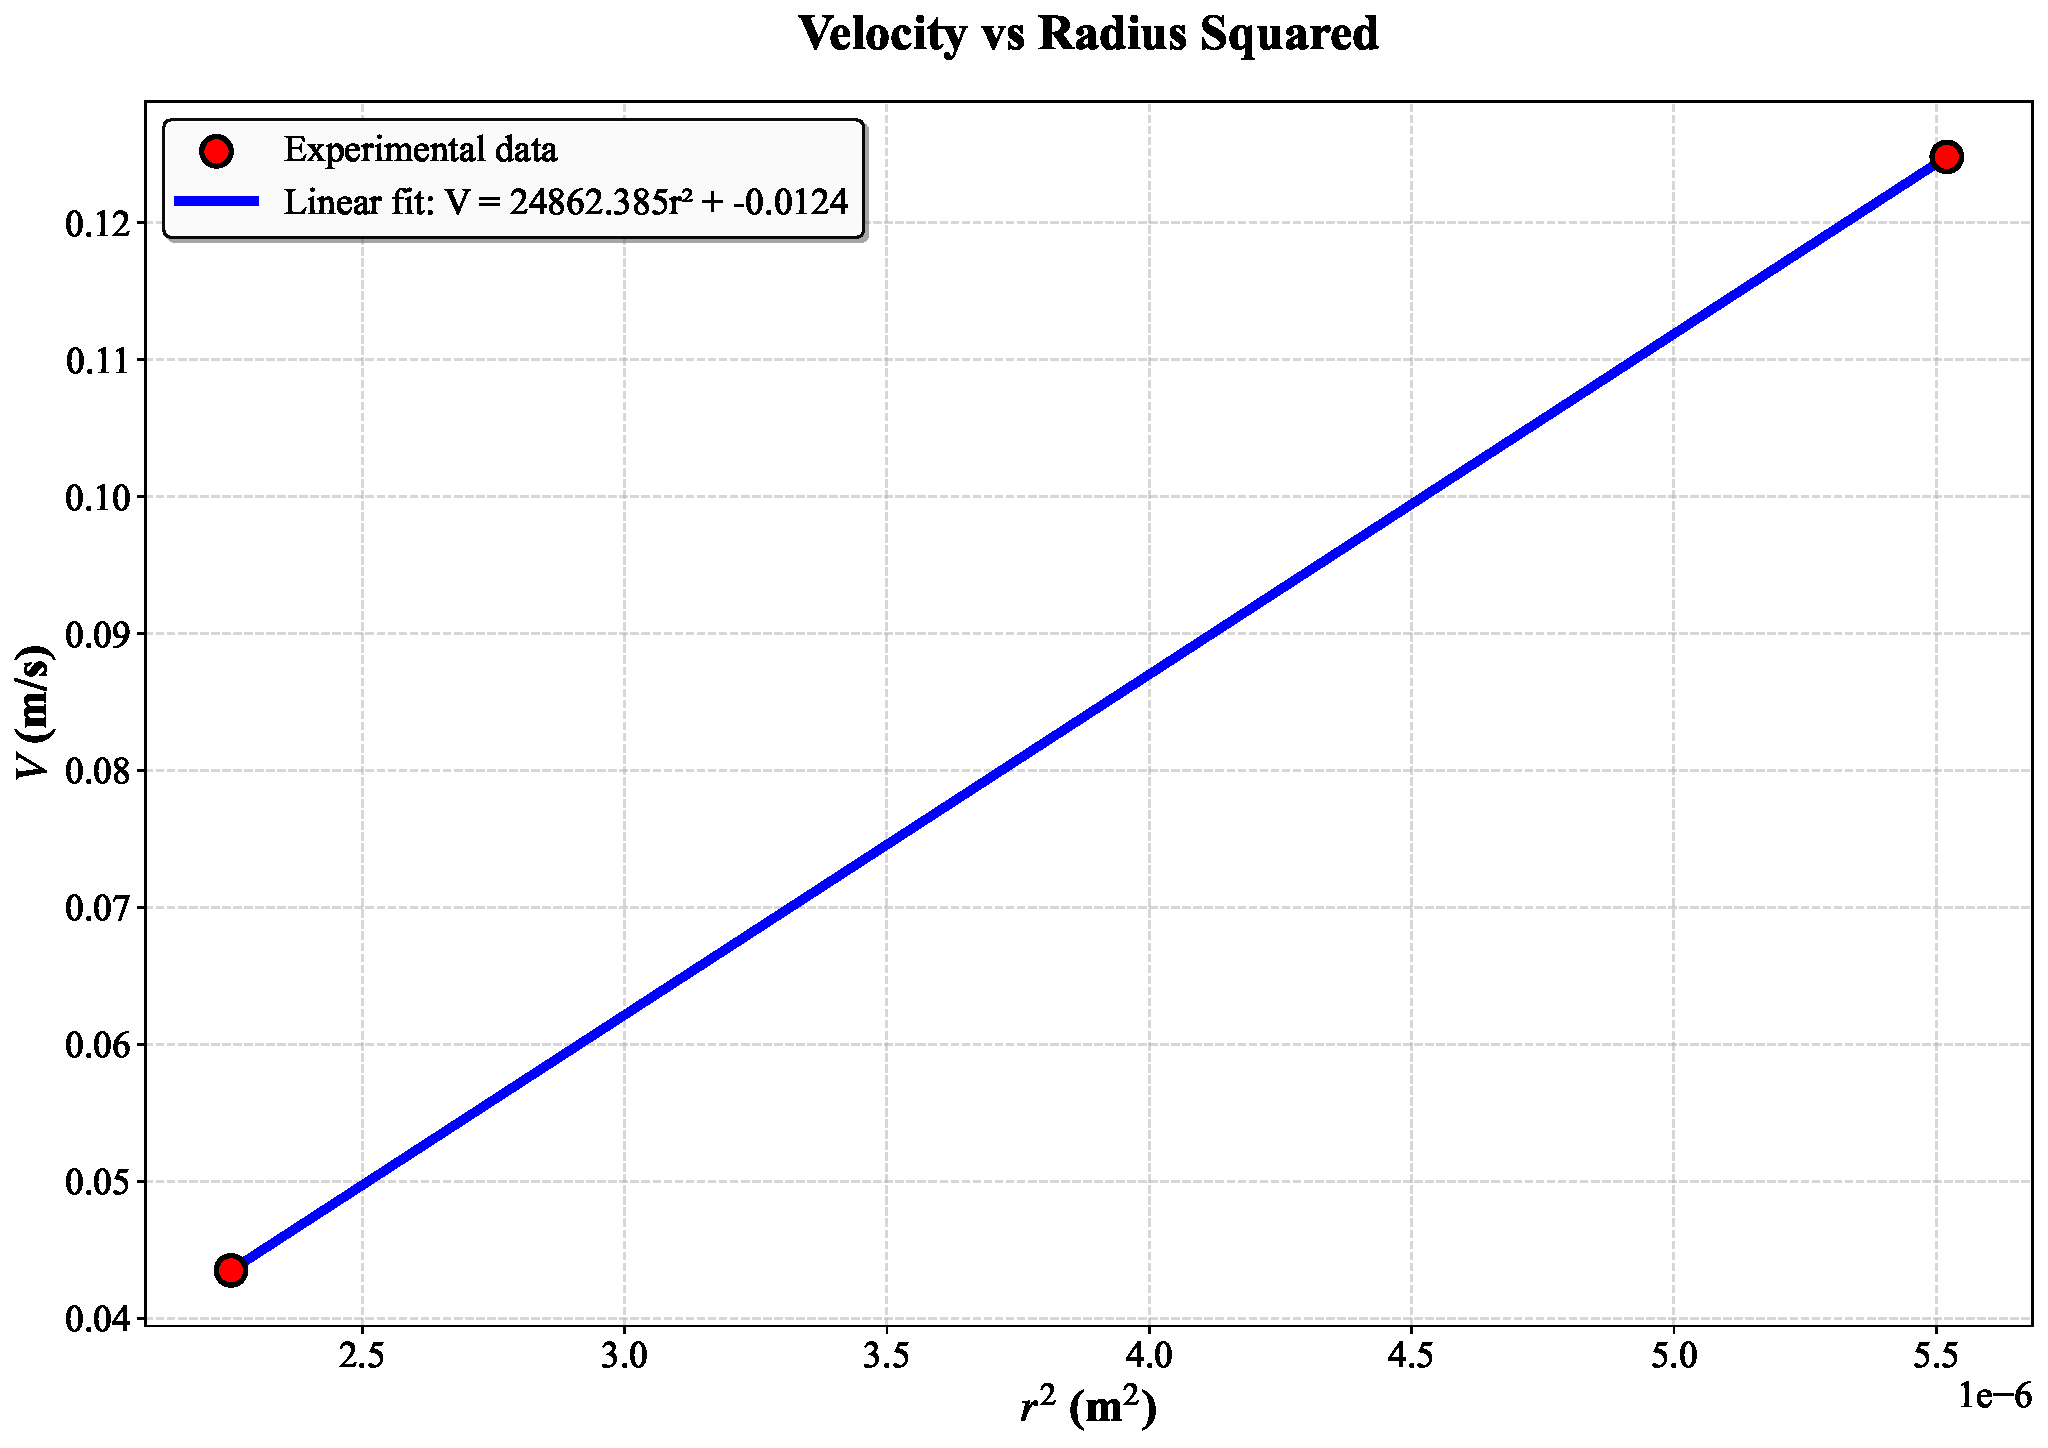
\includegraphics[width=0.8\textwidth]{velocity_vs_radius_squared.pdf}
	\caption{$v$ vs. $r^2$ graph}
\end{figure}

\section{Error Analysis}
1. Percentage error for $\eta_{\text{avg}}$ compared to literature value at 20°C (approximately 1.41 Pa·s for pure glycerin):
\[ \% \text{ error} = \left| \frac{0.7284 - 1.41}{1.41} \right| \times 100 \approx 48.3\% \]

2. The relative error formula derived from $\eta = \frac{2}{9} \frac{(\rho_2 - \rho_1) g r^2}{v}$, with $v = L / t$:
\[ \frac{\Delta \eta}{\eta} = \frac{\Delta (\rho_2 - \rho_1)}{|\rho_2 - \rho_1|} + \frac{\Delta g}{g} + 2 \frac{\Delta r}{r} + \frac{\Delta t}{t} + \frac{\Delta L}{L} \]
Assuming $\Delta g = 0$, and densities known precisely for this calculation, it simplifies to:
\[ \frac{\Delta \eta}{\eta} \approx 2 \frac{\Delta r}{r} + \frac{\Delta t}{t} + \frac{\Delta L}{L} \]

3. Maximum absolute errors:
- For radius: caliper precision $\Delta d = 0.01$ cm, so $\Delta r = 0.005$ cm.
  - Ball 1: $\Delta r / r = 0.005 / 0.235 \approx 0.021$
  - Ball 2: $\Delta r / r = 0.005 / 0.150 \approx 0.033$
- For time: stopwatch human error $\Delta t \approx 0.1$ s.
  - Ball 1: $\Delta t / t_{\text{avg}} = 0.1 / 0.593 \approx 0.169$
  - Ball 2: $\Delta t / t_{\text{avg}} = 0.1 / 1.70 \approx 0.059$
- For length: ruler precision $\Delta L = 0.1$ cm = 0.001 m, $\Delta L / L = 0.001 / 0.074 \approx 0.014$

Maximum relative error for ball 1: $2 \times 0.021 + 0.169 + 0.014 \approx 0.225$ or 22.5\%, $\Delta \eta_1 \approx 0.6717 \times 0.225 \approx 0.151$ Pa·s

For ball 2: $2 \times 0.033 + 0.059 + 0.014 \approx 0.139$ or 13.9\%, $\Delta \eta_2 \approx 0.7851 \times 0.139 \approx 0.109$ Pa·s

4. Average standard deviation of $\eta$ values (using the two $\eta$):
\[ s = \sqrt{ \frac{ \sum (\eta_i - \eta_{\text{avg}})^2 }{N-1} } = \sqrt{ \frac{ (0.6717 - 0.7284)^2 + (0.7851 - 0.7284)^2 }{1} } \approx 0.080 \, \text{Pa·s} \]

5. Possible causes of error:
- Impurity in glycerin (e.g., water absorption from humid air), leading to lower density and viscosity.
- Human error in timing, especially for faster balls.
- Wall effects if the cylinder is too narrow relative to ball size.
- Temperature fluctuations during the experiment.
- Limited number of balls and trials, reducing statistical accuracy.
- Assumption that terminal velocity is reached exactly at mark A.

\section{Results and Discussion}
In this experiment, we measured the viscosity coefficient of glycerin using Stokes' Law, obtaining an average value of $\eta_{\text{avg}} = 0.7284$ Pa·s at 20°C from direct calculations and $\eta_{\text{graph}} = 0.611$ Pa·s from the slope of the $v$ vs. $r^2$ graph. The corrected value at 18°C is approximately 0.766 Pa·s. These values are lower than the literature value for pure glycerin at 20°C, which is about 1.41 Pa·s, resulting in a percentage error of around 48.3\%.

The results confirm the theoretical prediction of Stokes' Law that terminal velocity is proportional to the square of the radius, as evidenced by the linear graph. However, the discrepancy between $\eta_{\text{avg}}$ and $\eta_{\text{graph}}$ highlights the limitations of using only two data points, which can amplify errors in slope calculation. Analytically, this suggests that increasing the number of balls with varied radii would improve the robustness of the graphical method, providing a better fit and reducing sensitivity to individual measurement errors.

The primary issue identified is the impurity of the glycerin, likely due to prolonged exposure to humid air, causing water absorption that dilutes the fluid and reduces both density (measured 900 kg/m³ vs. typical 1260 kg/m³) and viscosity. This problem is evidently present, as our values align more closely with those of glycerin-water mixtures (e.g., around 50-70% glycerin has viscosities in the 0.5-1 Pa·s range at 20°C). To mitigate this, future experiments should use freshly sealed glycerin and conduct the test in a controlled humidity environment. Additionally, measuring the actual density of the glycerin sample rather than using a assumed value would allow for more accurate comparisons.

Other errors, such as timing inaccuracies, could be addressed by using automated sensors or video recording for precise fall times. The wall effect, where proximity to cylinder walls increases drag, might be minimized by using a wider container. Although this is a standard lab experiment without novel methodologies, it provides valuable insight into fluid dynamics, emphasizing the importance of material purity in physical measurements. Overall, while the results deviate from pure glycerin values, they successfully demonstrate the principles of viscous drag and offer practical lessons on experimental precision and error mitigation, directing towards more refined techniques in advanced fluid studies.

\newpage

\textbf{Student Information}

Name Surname: Hakkı Erdem Günal

Student ID: 173223024

Course: Physics 3 Laboratory

Experiment No / Title: 2 / Viscosity Coefficient of Glycerin

Experiment Date: September 29, 2025

Submission Date: October 5, 2025

\end{document}